\section{Différents algorithmes de synthèse d'ouverture}
Cette section porte sur la présentation puis la comparaison des différents algorithmes de formation d'image de radar à synthèse d'ouverture. L'objectif est de réaliser un choix sur l'algorithme que nous allons utiliser. ...........
\subsection{$\omega-k$}

\begin{equation}
s_r(t, u)=\sum_{n}{A_{0}^{2}\sigma_{n}T_{p}e^{-j\Phi}\, \sin_{c}\!\left(KT_{p}\!\left(t-\frac{\sqrt{x_{n}^{2} + (y_{n} - u)^{2}}}{c}\right)\right)\, e^{-j2k\sqrt{x_{n}^{2} + (y_{n} - u)^{2}}}\, e^{j\omega t}}
\end{equation}

\begin{equation}
    S_{r}(\omega, k_{u}) = \sum_n A_{0}^2\sigma_{n}H_{r}(\omega) C(k, k_{u}).e^{-j\sqrt{4k^2-k_{u}^2}x_{n}}.e^{-jk_{u}y_{n}}
\end{equation}

\subsection{Backprojection}
L’algorithme de backprojection est une méthode fondamentale en imagerie radar, utilisée pour reconstruire des images haute résolution à partir des signaux radar acquis le long d’une trajectoire. Son principe repose sur l’exploitation de la cohérence de phase et de la diversité des angles d’observation offerte par le déplacement du radar. Pour chaque pixel de l’image à reconstruire, l’algorithme projette  les contributions des signaux reçus, en tenant compte de la distance et de la phase associée à chaque position du radar le long de sa trajectoire. En sommant de manière cohérente (prenant en compte la phase) ces contributions, les cibles réelles sont renforcées par interférence constructive, tandis que le bruit et les artefacts sont atténués.

\begin{figure}[htbp]
    \centering
    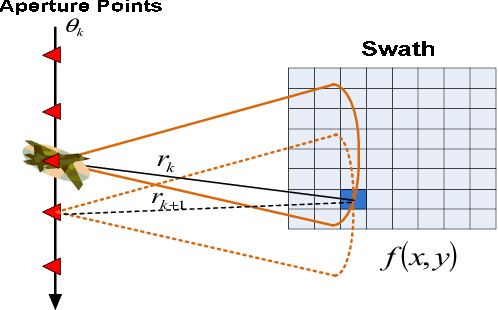
\includegraphics[width=0.5\linewidth]{src/rapport_complet/img/recouvrement_BP.png}
    \caption{Représentation du recouvrement en RSO}
    \label{fig:recouvrement_BP}
\end{figure}

Sur la Figure \ref{fig:recouvrement_BP}, on observe que, en raison du déplacement du drone et de l'ouverture de son antenne, certaines cellules au sol sont éclairées à plusieurs reprises le long de la trajectoire. Ce principe est à la base de l'amélioration de la résolution en imagerie SAR. En effet, chaque point de la scène est observé sous plusieurs angles successifs, ce qui permet d'exploiter la diversité des mesures. Les cibles réfléchissantes produisent alors des interférences constructives lors de la sommation cohérente, tandis que le bruit et les artefacts sont atténués par moyennage, améliorant ainsi le rapport signal-sur-bruit de l'image reconstruite. 

Techniquement, l'algorithme standard de Backprojection, pour chaque pixel, corrige uniquement la phase selon l'expression (\ref{eq:correction_bp})

\begin{equation}
    \label{eq:correction_bp}
    I(\Vec{p})=\sum_m s_{RC}(r_{\Vec{p}, m})e^{-j\varphi_{e}(r_{\Vec{p}, m})}
\end{equation}
Avec: 
\begin{description}
    \item{$s_{RC}(u_{m})$: Le signal reçu à une distance $u_{r}$ [m]}
    \item{$\varphi(u_{m})$: La phase attendue pour un signal à la distance $u_m$ [rad]}
\end{description}
Le terme $\varphi_e$ représente la correction de phase. 
La distance $r_{\Vec{p}, m}$ est une distance euclidienne. Par conséquent, cet algorithme ne réalise pas d'hypothèses sur la trajectoire du porteur. Dans le cadre de notre application, considérer une trajectoire quelconque est un grand avantage. 

Bien que cet algorithme soit conceptuellement simple, il est computativement exigeant, car il nécessite de parcourir chaque pixel de la scène et chaque position du radar. Cependant, sa robustesse et sa capacité à produire des images précises en font une référence pour les applications SAR, notamment lorsque la trajectoire du radar est irrégulière ou que la scène présente des reliefs complexes.
